\section{Hardware}
\label{sec:Hardware}

\newsavebox{\faceDiagram}
\sbox{\faceDiagram}	{
	\newcommand{\statcirc}[4]{
	\fill[opacity = 0.5, red,shift={(#1 cm,#2 cm)}, rotate=#3] (0,0) circle (#4); 
	\fill[opacity = 0.5, blue,shift={(#1 cm,#2 cm)},rotate=#3] (0,0) -- (180:#4) arc (180:0:#4) -- cycle;
	%	\draw[->,black,shift={(#1 cm,#2 cm)},rotate=#3] (#4, 0)
}

\newcommand{\drawArrow}[3]{
	\draw[->,>={Stealth[round]}, line width=0.75mm, black ,shift={(#1 cm,#2 cm)}, rotate=#3] (0,-0.5) -- (0,0.5); 
}

\newcommand{\drawchip}[3]{
	\tikzmath
	{
		\chipW = 0.35;
		\chipH = 0.4;
	}
	\fill[opacity = 0.75, darkgray, shift= {(#1 cm, #2 cm)}, rotate = #3, rounded corners] (-\chipH,-\chipW) rectangle (\chipH,\chipW);
	\fill[orange,shift= {(#1 cm, #2 cm)}, rotate = #3 ] (-0.25,0.2) circle (0.1);
}
\begin{tikzpicture}

	\tikzmath{
		\offsetAxis = 0.5;
		\offsetCent = 2.9;
		\diameter = 0.32;
	}
	\draw node (A) at (-0.5, 1.7) {};
	\draw node (B) at (0, 1.7) {};
	\drawchip{\offsetAxis}{\offsetCent}{0};
	\drawchip{-\offsetAxis}{-\offsetCent}{180};
	
	%Magnet North
	\statcirc{-\offsetAxis}{\offsetCent}{70}{\diameter};
	
	\drawArrow{-\offsetAxis}{\offsetCent}{70}
	
	%Magnet EAST
	\statcirc{\offsetCent}{\offsetAxis}{20}{\diameter};
	
	% Magnet West
	\statcirc{\offsetAxis}{-\offsetCent}{190}{\diameter};
	
	\statcirc{-\offsetCent}{-\offsetAxis}{45}{\diameter};
	
	\draw[gray, dashed] (-\offsetAxis,{\offsetCent + 1}) -- 
	(-\offsetAxis,{\offsetCent - 1});
	\draw[black,dotted] (0,0) circle (2.95);
	
	% 4 Cross Lines X
	\draw[black,dashed] (0,0) -- (4,0);
	\draw[black,dashed] (0,0) -- (-4,0);
	\draw[black,dashed] (0,0) -- (0,4);
	\draw[black,dashed] (0,0) -- (0,-4);
	
%	\draw[purple, dotted] ()
	% Dimensioned Variables
	\dimline[line style = {line width = 0.8, arrows = dimline reverse-dimline reverse}] {(A)}{(B)}{x};
	
	% Arc Radius
	\dimline[line style = {line width = 0.8}] {(0,0)} {++(150:2.95)}{R};
%	\dimline {(1,0)}{(-1,0)}{x};
\end{tikzpicture}
}

\newsavebox{\magnetDigitization}
\sbox{\magnetDigitization}	{
	
\newcommand{\statcirc}[4]{
	\fill[red,shift={(#1 cm,#2 cm)}, rotate=#3] (0,0) circle (#4); 
	\fill[blue,shift={(#1 cm,#2 cm)},rotate=#3] (0,0) -- (180:#4) arc (180:0:#4) -- cycle;
	%	\draw[->,black,shift={(#1 cm,#2 cm)},rotate=#3] (#4, 0)
}

\newcommand{\drawArrow}[3]{
	\draw[->,>={Stealth[round]}, line width=0.75mm, black ,shift={(#1 cm,#2 cm)}, rotate=#3] (0,-1) -- (0,1); 
}

\begin{tikzpicture}[scale = 0.75]
\tikzmath{
	\offsetAxis = 0.5;
	\offsetCent = 2.9;
	\diameter = 0.75;
}

\foreach \i in {1,...,30}
{
	\draw[gray] (0,0) -- (\i * 12-6 : 2.8);
	\node[inner sep=0pt] at (-{\i * 12}+12: 3) {\i};
}
\node[circle,draw,inner sep=0pt, fill = green] at (-{18 * 12}+12: 3) {18};
\statcirc{0}{0}{-204-90}{\diameter};
\drawArrow{0}{0}{-204-90};
\draw[black,dashed] (0,0) -- (3,0);
\draw[black,dashed] (0,0) -- (-3,0);
\draw[black,dashed] (0,0) -- (0,3);
\draw[black,dashed] (0,0) -- (0,-3);
\draw[gray, dotted] (0,0) -- (-204: 3);
\draw[gray, dotted] (0,0) -- (-204: 3);
\draw [white, line width = 5pt] (2.1,0)  arc (0:360-204:2.1);
\draw [<->, >={Stealth[round]}] (2.1,0)  arc (0:360-204:2.1);
\node[circle,inner sep=3pt, fill = white]				at (90:2) {$\theta$};
\end{tikzpicture}
}

%%%%%%%%%%%%%%%%%%%%
The \tagNamePlural were designed and tested with the M-Blocks modular robots as the test bed, although nothing precludes their use in other circumstances. In this section we breifly describe the M-Blocks hardware, and then describe the mechanical, and electrical aspects of the new \tagNamePlural.

\subsection{M-Blocks hardware overview}
\label{sec:mblocksOverview}

The \tagName were designed and tested with the M-Blocks modular robots as the test bed, although nothing precludes their use in other circumstances and [], called the 3d M-Blocks. Characteristics of the M-Blocks at a glance can be seen in Table~\ref{tab:hardwareOverview}

\subsection{\tagNamePlural Hardware Overview}
\label{sec:tagsOverview}
In order to create a tag where the reader and the tag are both ungendered...


\begin{figure*}[t]
	%\begin{tikzpicture}[minimum width = 14 cm, minimum height = 6 cm]
		%\draw (0,0) -- (14,6);
		
		\begin{tikzpicture}[]
		%complexnode/.pic={\usebox{\mybox}}]

		\newcommand\xa{2};
		\newcommand\xb{2};
		\newcommand\ya{2};
		\newcommand\yb{2};
		
		\coordinate (smallNE) at (2,5);
		\coordinate (smallSE) at (2,5);
		\coordinate (smallSW) at (2,5);
		\coordinate (smallNW) at (2,5);
		
		\coordinate (bigNE) at (2,5);
		\coordinate (bigSE) at (2,5);
		\coordinate (bigSW) at (2,5);
		\coordinate (bigSE) at (2,5);
		
		\node at (4 cm, 4 cm) {\usebox{\faceDiagram}};
		\node at (10 cm, 6 cm) {\usebox{\magnetDigitization}};
	
		
		%\draw (1,1) pic {complexnode} (4,4);
		
		\end{tikzpicture}
	%%%%%%%%%%%%%%%%%%%%%%%%%%%%%%%%%%%%%%%%%%%%
	\caption{TEXT GOES HERE $\pi$ /2 4 way symmetric layout}
	\label{fig:tagDiagram8}
\end{figure*}


\begin{figure}[b]
%%%%%%%%%%%%%%%%%%%%%%%%%%%%%%%%%%%%%%%%%%%%
	
\newcommand{\statcirc}[4]{
	\fill[red,shift={(#1 cm,#2 cm)}, rotate=#3] (0,0) circle (#4); 
	\fill[blue,shift={(#1 cm,#2 cm)},rotate=#3] (0,0) -- (180:#4) arc (180:0:#4) -- cycle;
	%	\draw[->,black,shift={(#1 cm,#2 cm)},rotate=#3] (#4, 0)
}

\newcommand{\drawArrow}[3]{
	\draw[->,>={Stealth[round]}, line width=0.75mm, black ,shift={(#1 cm,#2 cm)}, rotate=#3] (0,-0.5) -- (0,0.5); 


}

\newcommand{\drawchip}[3]{
	\tikzmath
	{
		\chipW = 0.35;
		\chipH = 0.4;
	}
	\fill[ black, shift= {(#1 cm, #2 cm)}, rotate = #3 ] (-\chipH,-\chipW) rectangle (\chipH,\chipW);
	\fill[ orange,shift= {(#1 cm, #2 cm)}, rotate = #3 ] (-0.25,0.25) circle (0.125);
	
}

\begin{tikzpicture}
\tikzmath{
	\offsetAxis = 0.5;
	\offsetCent = 2.9;
	\diameter = 0.32;
}

\drawchip{\offsetAxis}{\offsetCent}{0};
\drawchip{-\offsetAxis}{-\offsetCent}{180};
\statcirc{-\offsetAxis}{\offsetCent}{30}{\diameter};
\drawArrow{-\offsetAxis}{\offsetCent}{30}
\statcirc{\offsetCent}{\offsetAxis}{210}{\diameter};
\statcirc{\offsetAxis}{-\offsetCent}{190}{\diameter};
\statcirc{-\offsetCent}{-\offsetAxis}{45}{\diameter};
\draw[gray, dashed] (-\offsetAxis,{\offsetCent + 1}) -- 
(-\offsetAxis,{\offsetCent - 1});
\draw[black,dotted] (0,0) circle (3);
\draw[black,dashed] (0,0) -- (4,0);
\draw[black,dashed] (0,0) -- (-4,0);
\draw[black,dashed] (0,0) -- (0,4);
\draw[black,dashed] (0,0) -- (0,-4);
\end{tikzpicture}
%%%%%%%%%%%%%%%%%%%%%%%%%%%%%%%%%%%%%%%%%%%%
	\caption{tags consist of 4 diametrically magnetized
	magnes arranged in a $\pi$ /2 4 way symmetric layout}
	\label{fig:tagDiagram}
\end{figure}

%\begin{figure}[b]
%	%%%%%%%%%%%%%%%%%%%%%%%%%%%%%%%%%%%%%%%%%%%%
%	
\newcommand{\statcirc}[4]{
	\fill[red,shift={(#1 cm,#2 cm)}, rotate=#3] (0,0) circle (#4); 
	\fill[blue,shift={(#1 cm,#2 cm)},rotate=#3] (0,0) -- (180:#4) arc (180:0:#4) -- cycle;
	%	\draw[->,black,shift={(#1 cm,#2 cm)},rotate=#3] (#4, 0)
}

\newcommand{\drawArrow}[3]{
	\draw[->,>={Stealth[round]}, line width=0.75mm, black ,shift={(#1 cm,#2 cm)}, rotate=#3] (0,-1) -- (0,1); 
}

\begin{tikzpicture}[scale = 0.75]
\tikzmath{
	\offsetAxis = 0.5;
	\offsetCent = 2.9;
	\diameter = 0.75;
}

\foreach \i in {1,...,30}
{
	\draw[gray] (0,0) -- (\i * 12-6 : 2.8);
	\node[inner sep=0pt] at (-{\i * 12}+12: 3) {\i};
}
\node[circle,draw,inner sep=0pt, fill = green] at (-{18 * 12}+12: 3) {18};
\statcirc{0}{0}{-204-90}{\diameter};
\drawArrow{0}{0}{-204-90};
\draw[black,dashed] (0,0) -- (3,0);
\draw[black,dashed] (0,0) -- (-3,0);
\draw[black,dashed] (0,0) -- (0,3);
\draw[black,dashed] (0,0) -- (0,-3);
\draw[gray, dotted] (0,0) -- (-204: 3);
\draw[gray, dotted] (0,0) -- (-204: 3);
\draw [white, line width = 5pt] (2.1,0)  arc (0:360-204:2.1);
\draw [<->, >={Stealth[round]}] (2.1,0)  arc (0:360-204:2.1);
\node[circle,inner sep=3pt, fill = white]				at (90:2) {$\theta$};
\end{tikzpicture}
%	%%%%%%%%%%%%%%%%%%%%%%%%%%%%%%%%%%%%%%%%%%%%
%	\caption{tags consist of 4 diametrically magnetized
%		magnets arranged in a $\pi$/2 4 way symmetric layout}
%	\label{fig:tagDiagram}
%\end{figure}

\begin{table}[b]
  \caption{Basic info of the m-Blocks modular robots}

  \begin{tabular}{ p{3.4cm}  p{1.9cm} }
    \hline
    Actuation Directions & 6 \\
    Mass  & 150\,g \\
    Characterist Dimension & 50\,mm \\dra
    Total Parts  & 216 \\
    Actuated Moving Parts  & 10 \\
    Est. Cost & \$130 \\

  \end{tabular}

    \label{tab:hardwareOverview}
\end{table}


\subsection{Magnetic Barcodes Overview}
\label{sec:FlywheelAndBraking}

Several different Tag technologies are shown in Table~\ref{tab:info}.

More Text


%\begin{figure}[H]
%	\begin{tikzpicture}
%   	 \node[anchor=south west, inner sep=0] (image) at (0,0) {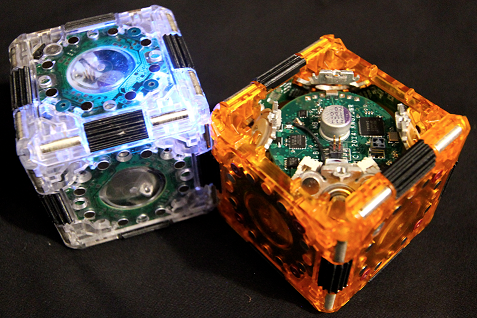
\includegraphics[width=2 in]{figures/cover.png}};
%    		\begin{scope}[x={(image.south east)},y={(image.north west)}]
%		%\node at (0.7,0.5) [align=center, rounded corners, fill=black!10, draw=none,opacity = 0.5]
%			%{$\omega = 0$\\$ V_{x} > 0 $\\ $ V_{y} = 0 $};
%		\draw[line width=1pt,->,red] (0.3,0.5) -- +(0:0.15);
%		\end{scope}
%	\end{tikzpicture}}
%\end{figure}


%%%%%%%%%%%%%%%%%%%%
%%%%%%%%%%%%%%%%%%%%
%%%%%%Old Text%%%%%%
%%%%%%%%%%%%%%%%%%%%%
%%%%%%%%%%%%%%%%%%%%%
%%%%%%%%%%%%%%%%%%%%%

%
%We have constructed four active 3D M-Blocks modules, as well as many
%passive modules. Although the modules share the basic shape and
%magnetic bonding mechanism as the previous one-dimensional system, almost % Mechanism? System? Interface? unsure what word here
%every part has been completely redesigned.  The significant changes  % As or like?
%include the plane changing mechanism, edge gear teeth, and simplified
%secondary magnet arrangement.  The basic parameters of the new module,
%and how they compare with the previous
%version, are shown in Table~\ref{tab:info}.
%
%\begin{table}[h]
%  \caption{Comparison of 3D M-Blocks to first generation M-Blocks. $ \dagger$ Pre-assembled ball bearings and assembled printed circuit boards are counted as single parts.}
%
%  \begin{tabular}{ p{3.4cm}  p{1.9cm}  p{1.9cm} }
%    \hline
%    & M-Blocks & 3D M-Blocks \\
%    \hline
%    Actuation Directions & 1 & 6 \\
%    Mass & 143\,g & 150\,g \\
%    Flywheel Moment of Inertia & 5.7\,E-6\,$\text{kgm}^2$ & 8.4\,E-6\,$\text{kgm}^2$ \\
%    Total Parts $ \dagger$ & 178 & 216 \\
%    Actuated Moving Parts  & 8 & 10 \\
%    Unique Parts & 30 & 46 \\
%    Est. Cost & \$250 & \$130 \\
%    Maximum Torque & 1.6\,Nm & 2.6\,Nm \\
%  \end{tabular}
%
%  \label{tab:info}
%\end{table}
%
%
%The goal of redesigning the M-Blocks was to extend their functionally
%to three dimensions while maintaining robustness and keeping the
%components as simple and mass-producible as possible. In order to
%extend the original M-Blocks concept to three planes, we first
%considered three separate, mutually orthogonal inertial actuators,
%similar to the design for Cubli~\cite{Cubli}.  However it proved
%difficult to fit three separate sets of flywheels, motors, and brakes
%inside the 50\,mm modules while maintaining a torque density sufficient to perform lattice % changed from torque - to moment - of - inertia ratio
%reconfiguration. Despite the added complexity of having to change planes, the advantage in power of a larger single
%flywheel proved to be the better solution.
%
%The redesign has focused on replacing complex actuators with simple
%ones while also attempting to utilize under-actuation where
%possible. For example, the flywheel brake in the 3D M-Blocks is built
%from a coil, two magnets, and a simple linkage.  In contrast, the
%original M-Blocks employed a hobby-style servo motor which was large
%and prone to failure.  Additionally, the orientation of the flywheel
%with respect to the module's frame is now controlled
%by the primary inertial actuator and a locking mechanism instead of an additional motor.
%
%While the 3D M-Blocks have more parts and more mass than their
%predecessors, they are capable of producing a higher maximum torque,
%controlled by more robust and capable electronics, and require less expensive machining.  The modules have proven to be robust,
%undergoing hundreds of reconfiguration movements without degradation,
%and surviving many falls of up to one meter in height.  The remainder
%of this section will describe the mechanical structure of the modules,
%the design of the inertial actuator, the operation of the plane
%changing mechanism, and the details of the electronics which control
%the modules.
%
%%%%%%%%%%%%%%%%%%%%%%%%%%%%%%%%%%%%%%%%%%
%\subsection{Overall Module Design}
%%%%%%%%%%%%%%%%%%%%%%%%%%%%%%%%%%%%%%%%%%
%
%\begin{figure*}[t*]
%
%  \centering
%  \includegraphics[width=6in]{Figures/ExplodedViewWithInsets.png}
%
%  \caption{Each 3D M-Block is built around a six-piece injection
%    molded frame \emph{gray} which supports the central assembly  \emph{lighter
%    gray, split in half} along the frame's longest diagonal axis on
%    two ball bearings  \emph{pink}. The molded frame holds eight magnets colored red and
%blue to represent their magnetic
%polarities. The central assembly holds batteries
%     \emph{yellow} and circuit boards  \emph{green} as well as the flywheel
%     \emph{purple}. The flywheel represents the inertial actuator.  For
%    clarity, the brake assembly is not shown in the exploded-view, it
%    can be seen in the bottom-left inset picture.  The top-right inset
%    picture shows the main PCB.}
%
%  \label{fig:ExplodedView}
%\end{figure*}
%
%
%The 3D M-Blocks consist of four primary mechanical assemblies: a frame
%(1) which holds the central assembly (2) which in turn supports the
%flywheel (3) and the braking mechanism (4).  In addition, the central
%assembly holds the four batteries which power the module and two of
%the printed circuit boards (PCBs) which control it.  The exploded
%view in Figure~\ref{fig:ExplodedView} shows the frame, central
%actuator, flywheel, batteries, and control PCBs.  The two insets in
%Figure~\ref{fig:ExplodedView} show actual photos of the finalized
%central assembly with all components including the braking system.  The braking mechanism is omitted from the exploded view
%because it is shown in better detail in Figure~\ref{fig:Brake}.
%
%At the core of the central assembly is a brushless motor and flywheel
%which, together with the braking mechanism, generate the torques
%required for all module movements and central assembly plane changes.
%The entire central assembly is supported by two ball
%bearings on a diagonal rotational axis which extends through two
%opposite corners of the cubic frame.  As the central actuator rotates
%about this diagonal axis, the flywheel aligns with each of the
%module's coordinate axes.
%
%%%%%%%%%%%%%%%%%%%
%\subsection{Frame}
%\label{sec:Frame}
%%%%%%%%%%%%%%%%%%%
%
%The 50\,mm cubic frame is built from six identical injection-molded
%panels which snap together.  Each panel contains two functional edges which contain two diametrically
%magnetized cylindrical magnets. Furthermore, each panel holds eight smaller
%alignment magnets in the faces.  The details of this magnetic interface configuration are described in
%~\cite{RomanishinRus-IROS13}. This magnetic interface
%allows neighboring modules to pivot about the cylindrical magnets in
%their common edges, and to form face to face bonds.
%
%In the 3D M-Blocks, we have added 15\,mm wide sections of gear teeth
%along each module's edges (shown in black in
%Figure~\ref{fig:ExplodedView}).  These gear teeth prevent slippage as
%two modules pivot relative to one another.  Because the shape of the gear teeth does not
%protrude past the extents of the frame, it does not hinder
%the ability of modules to pivot next to adjacent stationary modules.
%
%Finally, each frame panel holds a face PCB which is used to interface with the
%surrounding environment.
%
%Each of the eight corners of the frame contains an aluminum corner
%brace.  These braces are cut from sheet metal and die-formed so that
%they can be rigidly attached to the three adjacent panels.  In addition to
%adding strength to the frame, two of these corner braces provide rigid
%mounting points for ball bearings which connect the central assembly
%to the frame.  Three additional corner braces contain specialized
%mating holes and magnets which are a part of the plane changing
%mechanism detailed in Section~\ref{sec:PlaneChanging}.
%
%%%%%%%%%%%%%%%%%%%%%%%%%%%%%%%%%%%%%%%%%%%%
%\subsection{Inertial Actuator Design}
%\label{sec:FlywheelAndBraking}
%%%%%%%%%%%%%%%%%%%%%%%%%%%%%%%%%%%%%%%%%%%%
%
%The inertial actuator consists of a flywheel and a self-tightening
%band brake. All of the relevant components which form the actuator are
%illustrated in Figure~\ref{fig:Brake}.
%
%\begin{figure}[htb]
%
%  \centering
%  \includegraphics[width=3.25in]{Figures/brake.png}
%
%  \caption{The inertial actuator operates by quickly decelerating a
%    spinning flywheel \emph{purple} with a neoprene belt \emph{dark gray} that
%    wraps around the flywheel and which is anchored in two
%    arms \emph{yellow}.  The belt is tightened by a linkage
%    \emph{green}, which is supported by ball bearings \emph{pink}, and which acts as a lever to amplify the force felt at the belt (\emph{blue} and \emph{red}  arrows indicated relative motions for both CW and CCW braking actions).  To activate the brake, the coil \emph{orange} briefly generates either a positive or negative magnetic field
%    which exerts a corresponding force on the two magnets \emph{red/blue} which drives the linkage. }
%
%  \label{fig:Brake}
%\end{figure}
%
%The flywheel assembly consists of a thin brass ring with an outer diameter of
%38.0\,mm, inner diameter of 34.0\,mm and a thickness of 10.5\,mm into which the motor's rotor is press-fit.
%This flywheel-rotor assembly is then connected by two bearings, one on
%either side of the stator, to the surrounding frame such that the
%flywheel is completely supported and not cantilevered.  This design
%allows for the motor and flywheel to have a thin profile while
%maintaining a stiff attachment to the frame.  The downside to this
%approach is that the three wires which power the stator must fit
%through the center of the bearings, thereby complicating the assembly
%process.
%
%Once the flywheel is spinning, the 3D M-Blocks use a direct drive
%electromagnetic coil actuator as shown in Figure~\ref{fig:Brake} to activate
%the brake.  We chose this approach for its fast linear response
%(10\,ms), adequate force (3\,N), bidirectionality, low cost, robustness,
%and size.
%
%To exert a torque on the 3D M-Block, the motor first accelerates the flywheel
%to a set speed.  With the motor coasting, the module energizes the
%pancake-shaped coil with 280 turns of \#30 AWG wire to create a magnetic
%field.  This magnetic field exerts forces on the two ring magnets and associated keeper, with one of the magnets attracted towards the center of the coil and the
%other repelled.  The resulting force is transferred and magnified by a ratio of two to one by the
%four-bar linkage to the belt-holder arms. The two belt-holder arms
%are each attached in a one-way lever configuration to their respective
%elements in the four-bar linkage, thus allowing for bi-directional
%motion, despite the physical constraints of the belt-arms. With one
%of the belt holder arms pulling on its end of the belt, the mechanism
%tightens the belt around the flywheel.  The other end of the belt is
%immobilized by a mechanical hard stop.
%
%The current flowing through the coil is always polarized such that the end
%of the belt which is pulled causes the belt to constrict in the same
%direction that the motor is spinning.  As the belt comes into contact
%with the flywheel, the friction between the two surfaces causes the
%belt to self-tighten and completely arrest the flywheel in a matter of
%milliseconds.
%
%This system represents a complete redesign from the previous
%iteration.  The redesign was necessary in order to fit the inertial
%actuator within the spherical constraint imposed on the design.  As
%part of the redesign, the flywheel has been made larger, thicker, and,
%as a result, has a higher moment of inertia which allows
%for larger peak torques to be applied to the module.  The flexible
%neoprene belt used for braking is now 25\% wider and 30\%
%longer, which increases its surface area, resulting in
%increased stopping power with less belt wear.
%
%
%%%%%%%%%%%%%%%%%%%%%%%%%%%%%%%%%%%%%%
%\subsection{Plane Changing Mechanism}
%\label{sec:PlaneChanging}
%%%%%%%%%%%%%%%%%%%%%%%%%%%%%%%%%%%%%%
%
%The central assembly in each 3D M-Block can be thought of as a sphere
%rotating inside of a cube (the frame). In order to fully
%constrain the two assemblies together three points of contact are
%required. Two of these points are formed by ball bearings attaching
%the central assembly to the frame through an axis aligned between two
%opposing corners of the frame (along the longest diagonal).  This
%diagonal axis is offset $35\pi/180$\,radians from that of the
%flywheel's axis of rotation.  This diagonal axis extends through two
%opposite corners of the cubic frame.  As the central actuator rotates
%every $2\pi/3$\,radians about this diagonal axis, the flywheel aligns
%with a different set of the module's faces.  That is, if the flywheel
%is initially aligned with the module's x-axis, rotating the central
%actuator by $2\pi/3$\,radians, in one direction or another, will bring the
%central actuator into alignment with the module's y- or z-axis.
%
%To lock the central assembly into place, a third connection point is
%necessary.  It is formed by a retractable pin which protrudes from the
%central actuator.  When extended, the pin mates with one of three
%matching holes in the frame's corner braces (see
%Figure~\ref{fig:PlaneChanging}).
%
%\begin{figure}[htb]
%
%  \centering
%
%  \begin{subfigure}[b]{.3\linewidth}
%    \includegraphics[width=1in]{Figures/FlywheelX.png}
%    \subcaption{X-axis}
%  \end{subfigure}
%  ~
%  \begin{subfigure}[b]{.3\linewidth}
%    \includegraphics[width=1in]{Figures/FlywheelY.png}
%    \subcaption{Y-axis}
%  \end{subfigure}
%  ~
%  \begin{subfigure}[b]{.3\linewidth}
%    \includegraphics[width=1in]{Figures/FlywheelZ.png}
%    \subcaption{Z-axis}
%  \end{subfigure}
%
%
%%%  \subfloat[X-axis]{\includegraphics[width=1.1in]{Figures/FlywheelX.png}}
%%%  \subfloat[Y-axis]{\includegraphics[width=1.1in]{Figures/FlywheelY.png}}
%%%  \subfloat[Z-axis]{\includegraphics[width=1.1in]{Figures/FlywheelZ.png}}
%
%  \caption{The 3D M-Block changes the alignment of its flywheel by
%    rotating the central assembly along a diagonal axis between two
%    opposite corners of the frame (pointing out of the page).
%    For every $2\pi/3$ radians of rotation along this axis, the
%    flywheel comes into alignment with a new axis of the frame.}
%

%  \label{fig:PlaneChanging}
%\end{figure}
%
%In order to switch planes, the 3D M-Block first spins-up the motor.  Once
%the flywheel has reached a constant speed, the pin is retracted, which allows the central assembly to spin freely on its diagonal
%rotation axis.  A torque is then generated by electronically braking
%the motor.  The component of this torque aligned with the diagonal axis, causes the central assembly to rotate and align with a new plane. Magnets, one embedded in
%the central assembly, and one next to each of the pin alignment holes
%in the frame, provide mechanical detents to assist with fine alignment
%between the central assembly and the frame.  Once the pin is aligned
%with one of the mating holes, it is then extended to lock the central
%assembly into place.
%
%
%%%%%
%%%%%
%%%%%
%%%%%
%%%%%
%
%During experiments with the 3D M-Blocks, we found that the central
%actuator sometimes stopped rotating about the diagonal axis at points
%which left the pin misaligned with the mating holes in the corners of
%the frame.  To combat this, we added additional repulsive magnets near
%one of the bearings which complement the attractive force already
%provided by the magnets near the pin mating holes.  While this change
%greatly reduced the frequency with which the central actuator ends up
%misaligned with the frame, it has also made it difficult for a module
%to change the plane of its central assembly if the module is not
%magnetically attached to a larger lattice.  Without additional mass to
%help immobilize the module, attempting to change the plane of the
%central actuator results in the entire module pivoting about one of
%its edges.  We plan to refine the magnet arrangement in
%order to eliminate this problem in the future.
%
%%%%%
%%%%%
%%%%%
%%%%%
%%%%%
%
%The retractable pin is controlled by a shape memory alloy (SMA) wire
%which contracts when heated.  The particular SMA wire is a 100\,mm long,
%0.25\,mm diameter FLEXINOL, which is contained within a heat-resistant,
%insulating PEEK plastic tube.  This tube insulates the wire from the
%metal structure of the central assembly, and it also allows the wire
%to bend a complete $\pi$\,radians in order to fit the necessary length of
%wire within a constrained area.  One end of the SMA wire is
%electrically connected to a constant current driver on the main
%circuit board.  The other end of the wire is crimped into the
%retractable pin, which touches the central aluminum frame, and
%provides an electrical ground.  A strong (425\,N/m) spring provides the
%necessary restoring force to extend the pin when the SMA is not being
%heated.  As such, the SMA only consumes current when the pin is being
%held in the retracted position.
%
%%%%%%%%%%%%%%%%%%%%%%%%%
%\subsection{Electronics}
%\label{sec:Electronics}
%%%%%%%%%%%%%%%%%%%%%%%%%
%
%The electronics, which control each 3D M-Block, are divided across eight
%different PCBs.  The core functionality comes from a main PCB attached
%to one side of the central actuator.  The main PCB holds a Nordic
%nRF51422 (nRF) microprocessor with an on-chip 2.4\,GHz radio.  The
%radio is capable of supporting both low-energy Bluetooth Smart (which
%we use for centralized control) and the ANT protocol (which we plan to
%use for module-to-module communication).  The nRF is connected via a
%two-wire bus to a 6-axis inertial measurement unit (IMU), the
%MPU-6050, produced by Invensense.  The IMU allows the nRF to determine
%the central actuator's orientation as it rotates.
%
%The central brushless motor control is managed by a dedicated Allegro
%MicroSystems A4960 which frees the main processor for higher-level
%tasks.  While the A4960 handles the low-level motor control,
%closed-loop speed regulation requires supervision from the nRF.  The
%A4960 can apply an electronic braking torque to the motor in order to
%decelerate it more slowly than the mechanical brake.
%
%The main PCB also includes circuitry to control the shape memory alloy
%(SMA) wire, which retracts the pin. The pin locks the central actuator
%into alignment with each of the 3D M-Block's coordinate planes.  The
%circuitry is based on a high-current LED driver and a low-side current
%sense amplifier. It is capable of driving a maximum of 1.5\,A through
%the SMA wire, but due to the relatively slow thermal response of the
%SMA, we modulate the current on and off to achieve sufficient force
%without overheating the SMA wire.  When retracting the pin, we apply
%an average of 1.2\,A for 2\,s, but once retracted, we have found
%that we only need to apply an average of 700\,mA to hold the pin
%stationary.
%
%Finally, the main PCB includes charging and balancing circuitry for
%the four 125\,mAh lithium-polymer batteries which power each 3D M-Block.
%The batteries are connected in series in order to supply sufficient
%voltage to drive the motor at speeds over 20,000\,RPM.  Charging is
%enabled by connecting the M-Block to a 5\,V, 500\,mA source (e.g. a USB
%port).  An on-board, current-limited boost converter controls the
%voltage and current delivered to the batteries.  If the nRF detects
%that one battery's voltage is exceeding that of the others, it
%switches in an additional resistive load across that battery thereby
%reducing its charge rate and keeping all batteries balanced.
%
%A battery protection IC independently monitors each battery's voltage
%and current drain and disconnects all batteries if it detects a fault
%condition.  The main PCB also includes additional reverse-voltage,
%over-current, over-temperature, and electrostatic discharge protection
%devices in recognition of the fact that the M-Blocks must remain
%robust when being deployed outside of the laboratory environment.
%
%To complement the main PCB, there is a daughter PCB attached to the
%opposite side of the central actuator.  The two PCBs communicate
%over the aforementioned two-wire bus with the nRF acting as the bus
%master.  In addition to providing the connection point for two of the
%four batteries, the daughter PCB holds the circuitry which drives
%current through the mechanical braking coil.  The braking circuitry is
%controlled by an STMicroelectronics STM32F051 microprocessor which is
%a slave on the two-wire bus.  The braking circuitry is based on an
%op-amp which linearizes a current-controlling PMOS device in order to
%provide continuous current control from 0 to 4\,A.
%
%The main and daughter PCBs are complemented by six face PCBs, which are
%embedded into each face of the frame.  At the moment, the face
%PCBs provide convenient electrical contacts through which to
%charge the batteries.  In the near future, Atmel ATtiny1634 processors
%on each of the face PCBs will enable infrared communication between
%neighboring M-Blocks.  There is also a footprint for a second IMU on
%the face PCBs so that the central actuator will be able to determine
%its position relative to that of the surrounding frame.  Like the
%processor on the daughter PCB, the Atmel processors will be slaves on
%the same two-wire communication bus.
%
%The face PCBs are electrically connected to the central assembly by
%custom slip rings formed by the bearings that support the central
%assembly.  One bearing is in direct electrical contact with the
%central assembly and provides a ground connection, while the other is isolated and carries one of the bus lines
%to the face PCBs.  We employ a brass pin, which
%passes through the center of the each bearing to carry 3.3\,V to the
%face PCBs.  The pin contacts a leaf spring soldered to one of the
%face PCBs.  Experiments have shown that the
%bearings present several Ohms of resistance. However, the face PCBs do not
%require high currents, so this is not problematic.
%When power is flowing into the central assembly during the charging process, the voltage drop
%across the bearings can be compensated for by an increase of the external
%charging voltage.
